\documentclass{article}
\usepackage{tabularx}
\usepackage{amsmath}
\usepackage{graphicx}
\usepackage[margin=2cm]{geometry}
\usepackage{cite}
\usepackage[final]{hyperref}
\usepackage{listings}
\usepackage{here}
\hypersetup{
	colorlinks=true,
	linkcolor=blue,
	citecolor=blue,
	filecolor=magenta,
	urlcolor=blue         
}

\begin{document}

\title{TP01\\Particles}
\author{Robin Faury}
\date{12/15/20}
\maketitle

\begin{abstract}
	In this practical work, we will see how to generate a cloud of particles and how to animate them in real time.
	\begin{figure}[h]
		\centering
		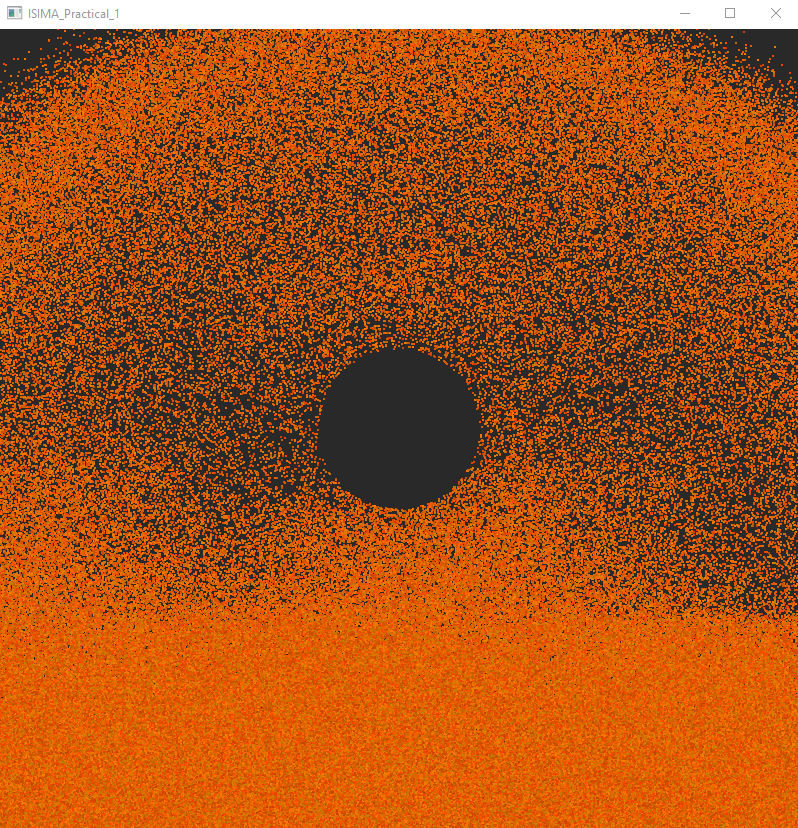
\includegraphics[scale=0.6]{images/result.png}
		\caption{A particle system}
	\end{figure}
\end{abstract}

\newpage
\section{Introduction}
\subsection{Cloning the repository}
You can find the source of the practical work by cloning this git repository:
\begin{lstlisting}
	https://github.com/robinfaurypro/GPGPU_ISIMA_2020-2021.git
\end{lstlisting}
The CMakeLists file is stored into the Practical\_1 folder. Open a terminal on this folder and use thus commands:
\begin{lstlisting}
	git submodule update --init
	mkdir build
	cd build
	cmake -G "Visual Studio 15 Win64" ..
\end{lstlisting}
Of course if you are on UNIX system feel free to use the generator you want.
If everything is going well, you can compile and run the executable and get a gray window.

\section{Original code}
On the main.cpp you can find all the code needed to render the current window. There are two shaders to display particles. The first one is named the vertex shader, it grab a collection of input buffers. The shader will be called for each particles we will create. The second shader is the fragment shader. it display particles and it will be called for each pixel on screen. We can see that the vertex shader can send to the fragment shader some information.\\
This process is know as the render pipeline. you start with some input buffers, thus buffers will be process by several shader (on per specific purpose) and finally print on a screen or a texture. This pipeline is static and optimized for rendering so it is NOT for a general purpose processing.
\begin{figure}[H]
	\centering
	
\includegraphics[scale=0.5]{images/rendering_pipeline.png}
	\caption{The graphic pipeline. Image from render doc application}
\end{figure}
The shader for general purpose processing is known as the Compute Shader. It only take buffers in inputs and it only release buffer in output. It is also a shader that can read AND write on the same buffer. Other shaders can but only with a very specific setup.
\begin{figure}[H]
	\centering
	
\includegraphics[scale=0.5]{images/compute_pipeline.png}
	\caption{The compute shader. Image from render doc application}
\end{figure}

The code remainder is quite straightforward:
\begin{itemize}
	\item Content: the structure to store our data
	\item Initialization: The initialization function (Compile our shaders)
	\item MoveParticles: The function to move to particles
	\item ComputeFrame: The function to call each frame
	\item Destroy: The function to clean up our data
	\item main: The main function to run the window
\end{itemize}

\section{GPU information}
On the Initialization function you can ask to your device what is its capability. For example, on the main function we check the version and the renderer. you can find here (\href{https://www.khronos.org/registry/OpenGL-Refpages/gl4/html/glGetString.xhtml}{https://www.khronos.org/registry/OpenGL-Refpages/gl4/html/glGetString.xhtml}) the list of properties. Check if the shading language version is 430 or more.\\
We need a 430 shading language version to run some compute shaders. We can now ask our GPU his compute capabilities using the glGetIntegeri OpenGL function:
\begin{lstlisting}
	int workgroup_count_x;
	glGetIntegeri_v(GL_MAX_COMPUTE_WORK_GROUP_COUNT, 0, &workgroup_count_x);
	// _v for vector (need to be called with 1 and 2 also to get the all vector)
\end{lstlisting}
Print the value of the vector GL\_MAX\_COMPUTE\_WORK\_GROUP\_COUNT, GL\_MAX\_COMPUTE\_WORK\_GROUP\_SIZE and the scalar GL\_MAX\_COMPUTE\_WORK\_GROUP\_INVOCATIONS.

\section{Particle buffer}
As you can see on the vertex shader, a particle is:
\begin{itemize}
	\item a 2D position
	\item a 2D velocity
	\item a color
	\item a life time
\end{itemize}
Create a struct to store of this values in this order and create a vector of Particule in the Content. For your information, glm::vec2 can store a 2D position or velocity. The particles vector can be initialize with 1024*1024 particles. Choose the start state of each particule. For example:
\begin{itemize}
	\item position = \{[0, 1], 0.9\}
	\item velocity = \{0, 0\}
	\item color = \{1, 0.5, 0\}
	\item life = 100
\end{itemize}
You can use the std::uniform\_real\_distribution function with 0 and 1 as parameters (normal distribution) to generate a rand number between 0 and 1.\\
Now we need to send our vector to the GPU. The GPU work with handle (a kind of pointer). Create a GLuint variable on the Content struct. and call the glGenBuffers.
\begin{lstlisting}
	glGenBuffers(1, &content.buffer_);
\end{lstlisting}
The first parameter is the number of buffer we need and the second is our handle. Add an assert after the call to check the value of content.buffer\_. It shouldn't be zero.\\
OpenGL work as a state machine. We can bind a buffer and all actions we will do will affect the binded buffer. Binding a buffer mean that we are working on it.
\begin{lstlisting}
	glBindBuffer(GL_SHADER_STORAGE_BUFFER, content.buffer_);
\end{lstlisting}
The first action to do is the allocation:
\begin{lstlisting}
	glBufferData(
		GL_SHADER_STORAGE_BUFFER,
		content.particles_.size()*sizeof(Particle),
		nullptr,
		GL_STATIC_DRAW);
\end{lstlisting}
Now we can ask a pointer on the data:
\begin{lstlisting}
	void *ptr = glMapBuffer(GL_SHADER_STORAGE_BUFFER, GL_WRITE_ONLY);
\end{lstlisting}
Adding the WRITE\_ONLY flag will help the driver. After the map action you can copy (with memcpy for example) your particle data. After that we must unmap the pointer.
\begin{lstlisting}
	void *ptr = glUnmapBuffer(GL_SHADER_STORAGE_BUFFER);
\end{lstlisting}
After this action the ptr variable isn't valid! Finally we can unbind the buffer.
\begin{lstlisting}
	glBindBuffer(GL_SHADER_STORAGE_BUFFER, 0);
\end{lstlisting}
On the ComputeFrame function uncomment the code. This is the call to the rendering pass. You should see this kind of result:
\begin{figure}[H]
	\centering
	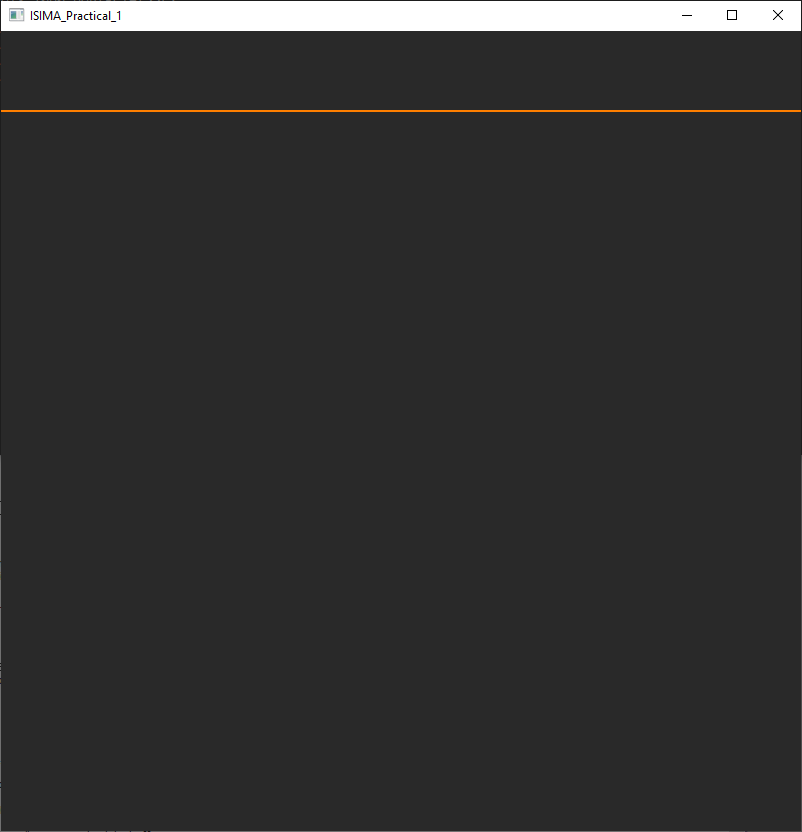
\includegraphics[scale=0.5]{images/init_buffer.png}
	\caption{Particles}
\end{figure}

\section{Move particle}
\subsection{CPU}
Firstable we need to write the process of moving the particle in CPU. Most of the time your algorithms must be write in C++ just in case the GPU your user use don't support compute shader. In this case we will use the CPU version as a comparison too. First, grab the GPU (device) buffer on the CPU (host) side using the glMapBuffer function and update the position and velocity of each particles using formulas below.
\begin{itemize}
	\item Bind the buffer
	\item Map the buffer using the GL\_READ\_WRITE option
	\item reinterpret cast the pointer into a Particle* pointer
	\item Update each particle
	\item Unmap the buffer
	\item Unbind the buffer
\end{itemize}

\begin{equation}
position_i = position_i + velocity_i * \Delta t + \frac{\Delta t^2*g}{2},
\end{equation}
\begin{equation}
velocity_i = g*\Delta t.
\end{equation}
With:
\begin{itemize}
	\item $\Delta t$: The time simulated between two frame (0.01 for example)
	\item $g$: The gravity \{0, -9.8\}
	\item $position_i$: The position of the particule i
	\item $velocity_i$: The velocity of the particule i
\end{itemize}
Before modify the buffer, you can check if the buffer uploaded on the GPU is correct (not fill with zeros).
\subsection{GPU}
\subsubsection{Shader}
Run the program and take a look at the FPS. A real time application should run at 16 ms per frame. For this 1 048 576 particles simulation we do not have this number. We need to find a way to optimize this. We can imagine using some std::thread but we can use the GPU and its 1000 cores to run 1000 threads.\\
The first thing to do is to create the compute shader. For that, create a new const char* variable like the vertex shader named kComputeSource. The first line of the shader is the version. After that copy paste your Particle struct in your shader. Now we can define the input buffer and its layout:
\begin{lstlisting}
	//...  (Version and Particle struct)
	layout(std140, binding=0) buffer Particles {
		Particle particles[];
	};
	//...
\end{lstlisting}
The input and output buffer is now named Particles and it is a vector of Particle. You can access to one particle through the variable particles[i].\\
Next you must specify the number of shader invocation. Remember that the shader can specify how many time it should be run. And because compute shader can compute data in 3D, you can specify a layout of invocation (a thread id can be in 3D).
\begin{lstlisting}
	//...
	layout(local_size_x = 128, local_size_y = 1, local_size_z = 1) in;
	//...
\end{lstlisting}
And finally the main function:
\begin{lstlisting}
	//...
	void main() {
		vec2 position = particles[gl_GlobalInvocationID.x].position_;
		vec2 velocity = particles[gl_GlobalInvocationID.x].velocity_;
		// ... (Move particle)
		particles[gl_GlobalInvocationID.x].position_ = position;
		particles[gl_GlobalInvocationID.x].velocity_ = velocity;
	}
	//...
\end{lstlisting}
Remember that gl\_GlobalInvocationID is the id of the thread so it's like the index of the particle in the vector.
You can re-implement your algorithm in this main program.
\subsubsection{Program}
We have now a shader code. We need to compile it and send it to the GPU. We need to make the same process as we did for the vertex shader.
\begin{itemize}
	\item Create a shader but with the GL\_COMPUTE\_SHADER flag
	\item Send the source
	\item Compile the source
	\item Check errors
\end{itemize}
Our shader must be wrapped inside a program. Add a Handle (GLuint) in the content struct to store the program name (kernel\_move\_particles\_ for example). The link of your program should return a valid handle. You can delete the shader, you just need the program.

\subsubsection{Dispatch}
We can now use the new compute program to move particles. In the MoveParticles function deactivate the CPU code (using \#if 0 or comment or a const bool) and use the compute program:
\begin{lstlisting}
	glUseProgram(content.kernel_move_particles_);
\end{lstlisting}
 As usual, you need to bind the particle buffer. But this time we also need to specify the binding location. On your shader you set binding=0:
\begin{lstlisting}
	glBindBufferBase(GL_SHADER_STORAGE_BUFFER, 0, content.buffer_);
\end{lstlisting}
And finally you can run the dispatch function:
\begin{lstlisting}
	glDispatchCompute(content.particles_.size()/128, 1, 1);
\end{lstlisting}
We set the number of particles divide by 128 because the layout value on x on the shader is 128.\\
The dispatch function will run the simulation asynchronous. To be sure to right measure the duration of the computation we need to add a synchronization point (a barrier). It is also very important to add a barrier if you dump data from the GPU just after a dispatch. You can grab just half of your buffer.
\begin{lstlisting}
	glMemoryBarrier(GL_SHADER_STORAGE_BARRIER_BIT);
\end{lstlisting}
After that we can clean the OpenGL state machine by disable the program:
\begin{lstlisting}
	glUseProgram(0);
\end{lstlisting}

\subsubsection{Destroy}
When the application is killed, we must clean our GPU resources. On the destroy function you need to delete the two program and the buffer:
\begin{lstlisting}
	glDeleteProgram(content.kernel_draw_particles_);
	glDeleteProgram(content.kernel_move_particles_);
	glDeleteBuffers(1, &content.buffer_);
\end{lstlisting}

\subsubsection{Results}
If everything is ok you should have this kind of result:
\begin{figure}[H]
	\centering
	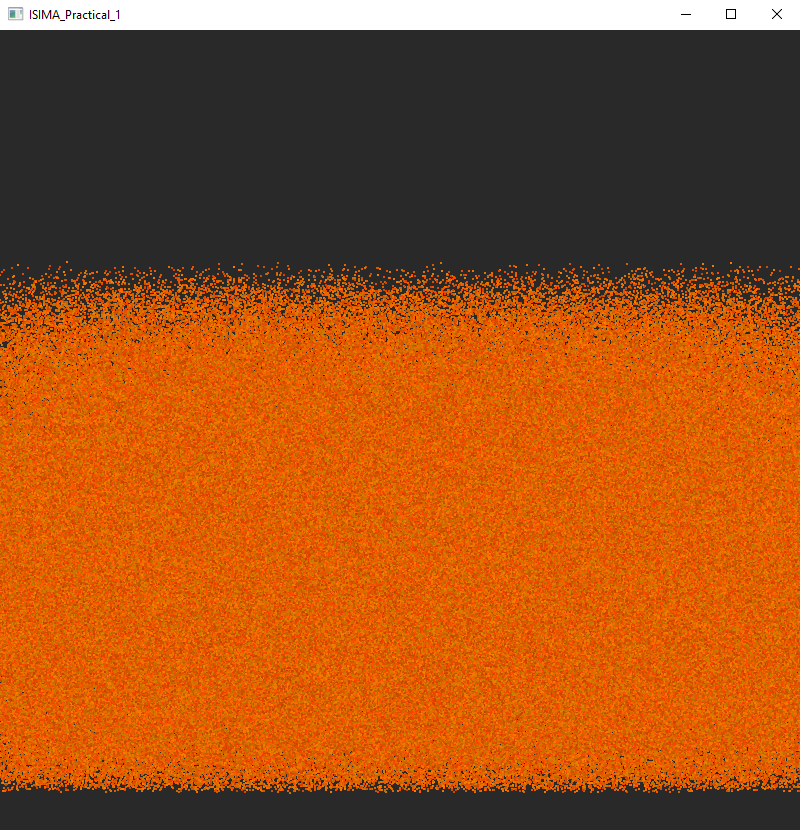
\includegraphics[scale=0.5]{images/result_simple.png}
	\caption{Particles falling}
\end{figure}
For this picture I set a random orange color for the color and a random velocity.\\

\section{Bonus}
We just simulate a atmosphere free domain. We can add a limit of the velocity on the shader.
\begin{lstlisting}
	velocity = clamp(velocity, -5.f, 5.f);
\end{lstlisting}
We saw that GPU doesn't have random function. But, we can simulate random function using sin function and magic number. On your compute shader add the random function above the main:
\begin{lstlisting}
	float random(vec2 st) {
		return fract(sin(dot(st.xy, vec2(12.9898, 78.233)))*43758.5453123);
	}
\end{lstlisting}

With this random function we can simulate a very rough ground. For that simply get a rand value from the position when the position is above 0 and compute the new velocity.
\begin{lstlisting}
	if (position.y < 0.0) {
		float rand = random(position);
		position.y = 0.0;
		velocity = -velocity; 
		vec2 normal = vec2(rand*2.0-1.0, 1.0);
		normal = normalize(normal);
		velocity = reflect(velocity, normal)*0.8;
	}
\end{lstlisting}

You can also add a circle on the middle of the screen. If the position less the center of the circle (0.5, 0.5) is less than the radius, then reflect the velocity with the normal of the sphere and recompute the position with the new velocity.

\section{Uniform value}
Some additional value can be add to our shader. It is called uniform. For example you can define: 
\begin{lstlisting}
	uniform float time;
\end{lstlisting}
and have access to the time variable in your shader code. you can set the time value on the CPU side after the glUseProgram:
\begin{lstlisting}
	glUniform1f(glGetUniformLocation(program_, "time"), glfwGetTime());
\end{lstlisting}
The time variable can be used to move the center of the sphere (using a sinus to keep the value between 0 and 1) for example.

\end{document}